\documentclass{resume}
\usepackage{graphicx}
\usepackage{hyperref}

\begin{document}

\contact{Sean C. Lewis}{(408) 470-0668}{\href{mailto:sean.phys@gmail.com}{sean.phys@gmail.com}}{\href{www.sc-lewis.com}{www.sc-lewis.com}}{\\}

\marginnote{
        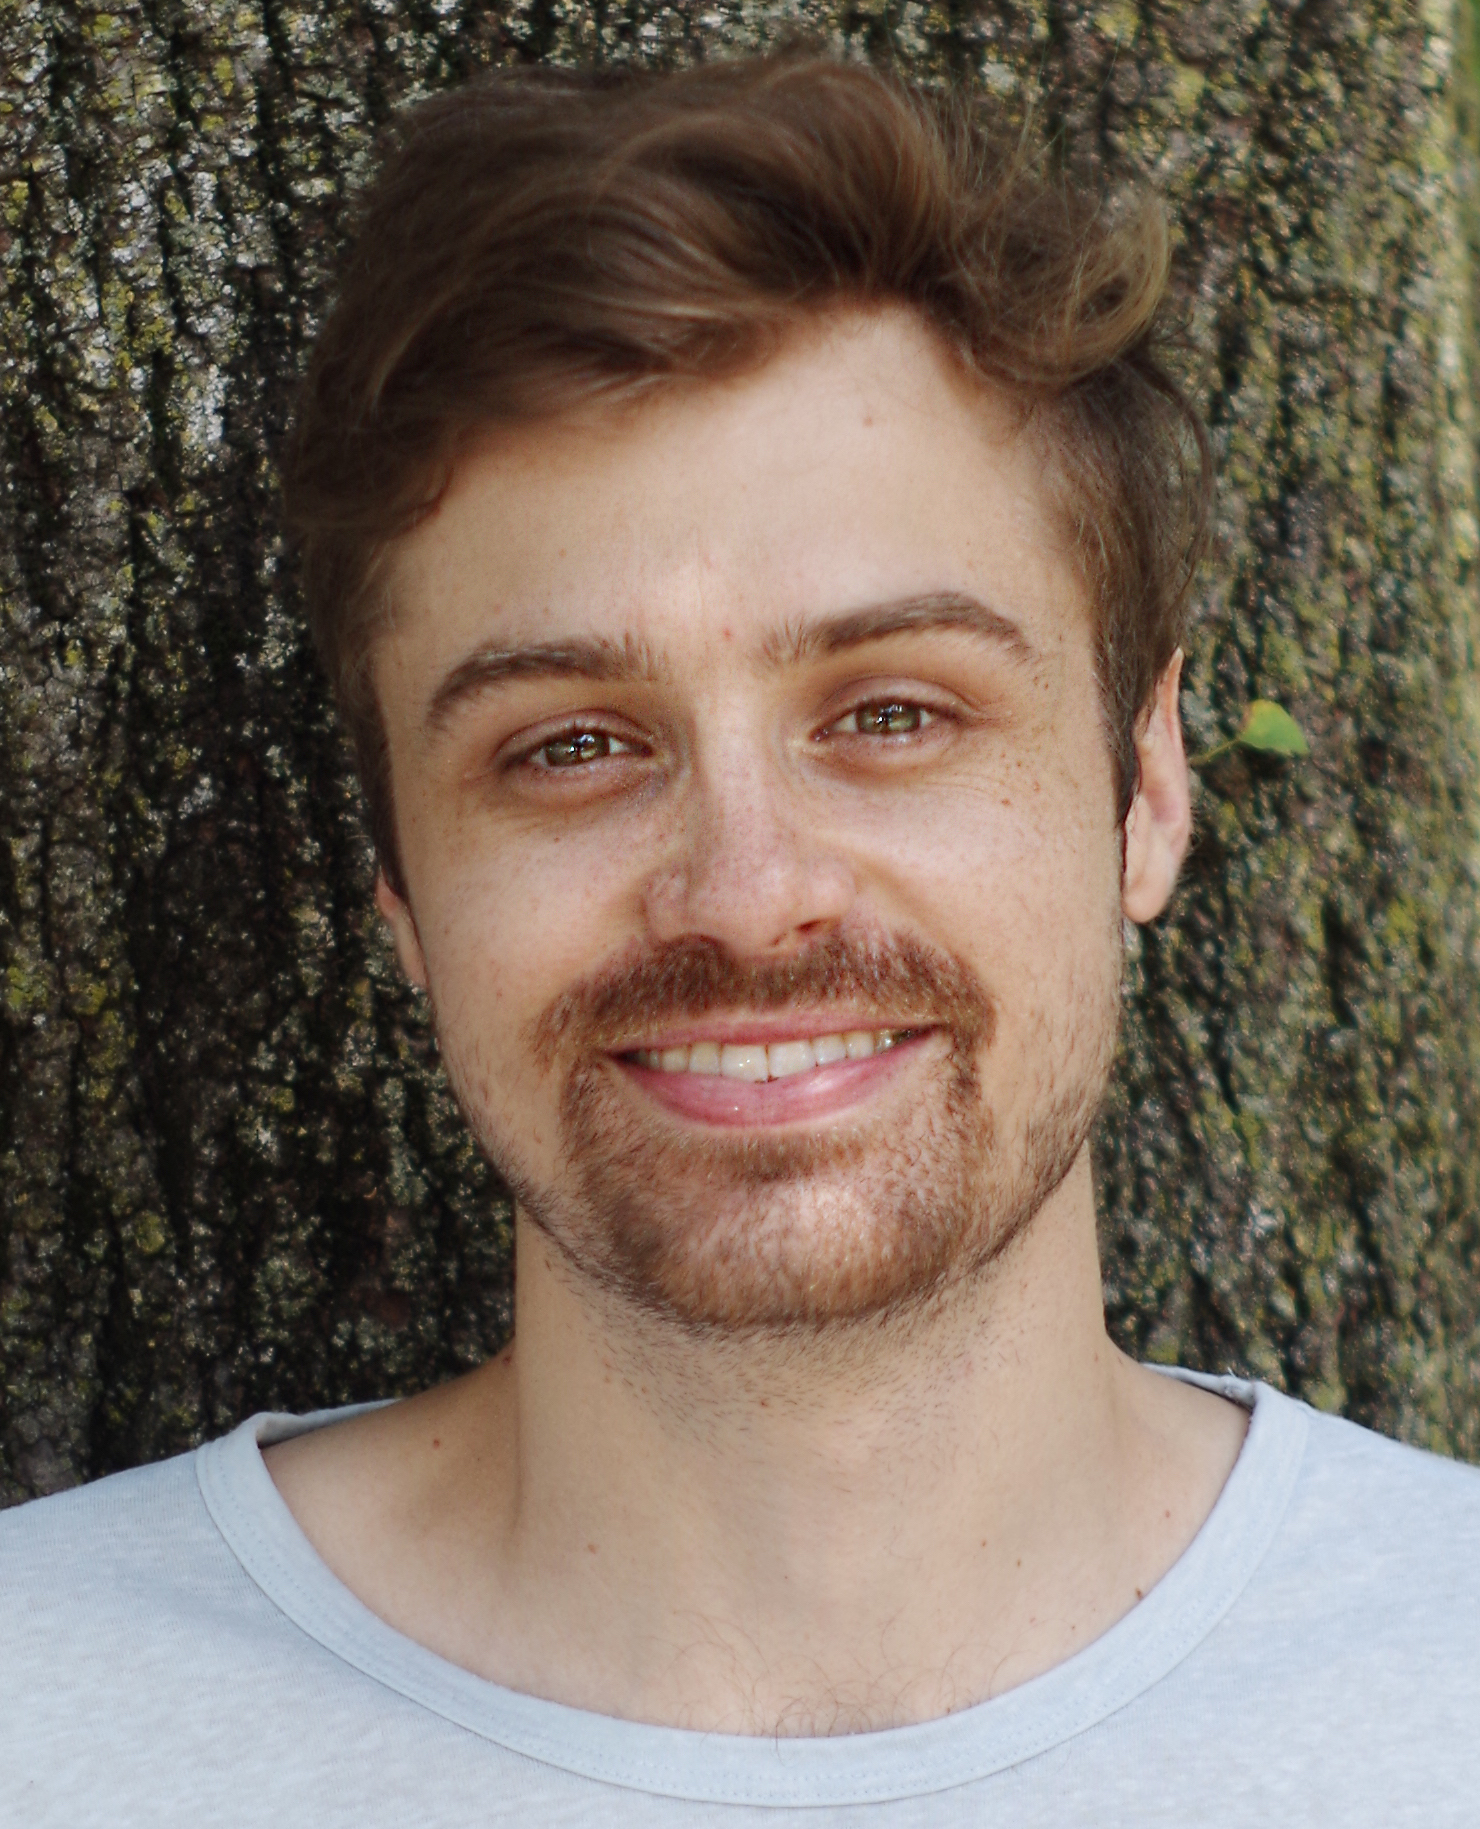
\includegraphics[width=5cm]{headshot2.jpg}
	\begin{skills}
		\bullet HPC Unix Systems
		\bullet Multiphysics Software Suites
		\bullet Software Design
		\bullet Data Analysis
            \bullet Machine Learning
            \bullet Git
	\end{skills}
	%
	\begin{languages}
		\bullet Python
		\bullet Fortran
		\bullet C
		\bullet HTML/CSS
            \bullet JavaScript
            \bullet Bash
	\end{languages}
        %
        \begin{interests}
            \bullet High Performance Computing
            \bullet Fluid Dynamics
            \bullet Software Development
        \end{interests}
}
\section*{\header{Education}}
\begin{education}{Ph.D. Physics}{Drexel University}{2023}
\end{education}

\begin{education}{M.S. Physics}{Drexel University}{2019}
\end{education}

\begin{education}{B.S. Physics}{California Polytechnic State University}{2016}{Cum Laude}
\end{education}

\section*{\header{Experience}}

\begin{job}{Drexel University}{Philadelphia, PA}{Research Fellow}{Aug 2019 -- Present}
	\bullet 
\end{job}

\begin{job}{Drexel University}{Philadelphia, PA}{Teaching Fellow}{Sept 2017 -- Present}
	\bullet Lead teaching sections for calculus-based Introductory Physics courses using progressive, science-based techniques.
	\bullet Received the Department of Physics Teaching Excellence Award in 2019 for outstanding student reviews and teaching practices.
\end{job}

\begin{job}{View Inc.}{Milpitas, CA}{Lab Tech Intern}{JUL -- SEP 2016}
	\bullet Calibrated instruments for product testing and development. Assisted in product performance analysis.
\end{job}

\section*{\header{Software Projects}}

\begin{project}{VorAMR}{Software Tool for Hydrodynamic Research}{https://bitbucket.org/torch-sf/vor-amr/src/main/}{Designed and deployed a novel method of translating data between hydrodynamical code-bases. }
\end{project}

\begin{project}{PythonOpenMPI}{Parallel Task-Based Processing Tool}{https://github.com/seanlabean/PythonOpenMPI}{Designed, deployed, and maintain an efficient python tool for data analysis parallelization via task-based methods.}
\end{project}

\begin{project}{GalDNN}{From-Scratch Deep Neural Network}{https://github.com/seanlabean/GalDNN}{Designed a proof-of-concept deep learning neural network that can accommodate any number of hidden layers and neurons within.}
\end{project}

\section*{\header{Talks \& Grants}}

\section*{\header{References}}

\begin{reference}{Stephen McMillan}{Ph.D. Advisor, Drexel University}
	(213) 555-0172\\
	morpheus@matrix.net
\end{reference}

\begin{reference}{Mordecai-Mark Mac Low}{Ph.D. Co-advisor, AMNH}
	(213) 555-0169\\
	theoracle@matrix.net
\end{reference}

\end{document}
